%%%%%%%%%%%%%%%%%%%%%%%%%%%%%%%%%%%%%%%%%%%%%%%%%%%%%%%%%%%%%%%%%%%%%%%%%
%  Zawartość: Praca Dyplomowa Inżynierska - System do obsługi laboratorium
%  fotograficznego z możliwością sprzedaży foto usług online.
%  Opracował: Adam Dłubak <adam.dlubak@gmail.com>
%  Data: Listopad 2017
%  Wersja: 1.0
%%%%%%%%%%%%%%%%%%%%%%%%%%%%%%%%%%%%%%%%%%%%%%%%%%%%%%%%%%%%%%%%%%%%%%%%%

\documentclass[a4paper,onecolumn,oneside,12pt,extrafontsizes]{memoir}
% W celu przygotowania wydruku do archiwum należy przesłonić komendę powyższą
% dwoma poniższymi komendami:
%\documentclass[a4paper,onecolumn,twoside,10pt]{memoir} 
%\renewcommand{\normalsize}{\fontsize{8pt}{10pt}\selectfont}

%\usepackage[cp1250]{inputenc} % jeśli kodowanie edytowanych plików to cp1250 
\usepackage[utf8]{inputenc} % jeśli kodowanie edytowanych plików to UTF8
\usepackage[T1]{fontenc}
\usepackage[polish]{babel}
%\DisemulatePackage{setspace}
\usepackage{setspace}
\usepackage{tabularx}
\usepackage{color,calc}
%\usepackage{soul} % pakiet z komendami do podkreślania tekstu

\usepackage{ebgaramond} % pakiet z czcionkami garamond, potrzebny tylko do strony tytułowej, musi wystąpić przed pakietem tgtermes

%% Aby uzyskać polskie literki w pdfie (a nie zlepki) korzystamy z pakietu czcionek tgterms. 
%% W pakiecie tym są zdefiniowane klony czcionek Times o kształtach: normalny, pogrubiony, italic, italic pogrubiony.
%% W pakiecie tym brakuje czcionki o kształcie: slanted (podobny do italic). 
%% Jeśli w dokumencie gdzieś zostanie zastosowana czcionka slanted (np. po użyciu komendy \textsl{}), to
%% latex dokona podstawienia na czcionkę standardową i zgłosi to w ostrzeżeniu (warningu).
%% Ponadto tgtermes to czcionka do tekstu. Wszelkie matematyczne wzory będą sformatowane domyślną czcionką do wzorów.
%% Jeśli wzory mają być sformatowane z wykorzystaniem innych czcionek, trzeba to jawnie zadeklarować.

%% Po zainstalowaniu pakietu tgtermes może będzie trzeba zauktualizować informacje 
%% o dostępnych fontach oraz mapy. Można to zrobić z konsoli (jako administrator)
%% initexmf --admin --update-fndb
%% initexmf --admin --mkmaps

\usepackage{tgtermes}   
\renewcommand*\ttdefault{txtt}

% We wcześniejszej wersji szablonu korzystano z innych czcionek. Dla celów historycznych pozostawiono je w komentarzu
%\usepackage{mathptmx} % pakiet będący następcą pakietów times and mathptm, niestety polskie literki są zlepkami
%\usepackage{newtxtext,newtxmath} % pakiety dostarczające Times dla tekstów i wzorów matematycznych,  
%                                  rozwiązuje problemy występujące w mathptmx, ale wymaga zainstalowania
%                                  dodatkowych pakietów oraz uruchomienia updmap (konsola administratora)
%                                  niestety polskie literki są zlepkami
%\usepackage{newtxmath,tgtermes} % można też połączyć czcionki do tekstu i czcionki do wzorów

\usepackage{listings} % pakiet do prezentacji kodu. 
%Wcześniej był problem z polskimi znakami w otoczeniu lstlisting, stąd pozostawiono w komentarzu zastosowane wtedy rozwiązanie: 
\lstset{literate=%-
{ą}{{\k{a}}}1 {ć}{{\'c}}1 {ę}{{\k{e}}}1 {ł}{{\l{}}}1 {ń}{{\'n}}1 {ó}{{\'o}}1 {ś}{{\'s}}1 {ż}{{\.z}}1 {ź}{{\'z}}1 {Ą}{{\k{A}}}1 {Ć}{{\'C}}1 {Ę}{{\k{E}}}1 {Ł}{{\L{}}}1 {Ń}{{\'N}}1 {Ó}{{\'O}}1 {Ś}{{\'S}}1 {Ż}{{\.Z}}1 {Ź}{{\'Z}}1 }%{\ \ }{{\ }}1}

% Choć możliwe jest zastosowanie różnych pakietów formatujących tabele, zaleca się tego nie robić.
%\usepackage{longtable}
%\usepackage{ltxtable}
%\usepackage{tabulary}

%%%%%%%%%%%%%%%%%%%%%%%%%%%%%%%%%%%%%%%%%%%%%%%%%%%
%% Ustawienia odpowiedzialne za sposób łamania dokumentu
%% i ułożenie elementów pływających
%%%%%%%%%%%%%%%%%%%%%%%%%%%%%%%%%%%%%%%%%%%%%%%%%%%
%\hyphenpenalty=10000		% nie dziel wyrazów zbyt często
\clubpenalty=10000      %kara za sierotki
\widowpenalty=10000  % nie pozostawiaj wdów
\brokenpenalty=10000		% nie dziel wyrazów między stronami
\exhyphenpenalty=999999		% nie dziel słów z myślnikiem
\righthyphenmin=3			% dziel minimum 3 litery

%\tolerance=4500
%\pretolerance=250
%\hfuzz=1.5pt
%\hbadness=1450

\renewcommand{\topfraction}{0.95}
\renewcommand{\bottomfraction}{0.95}
\renewcommand{\textfraction}{0.05}
\renewcommand{\floatpagefraction}{0.35}

%%%%%%%%%%%%%%%%%%%%%%%%%%%%%%%%%%%%%%%%%%%%%%%%%%%
%%  Ustawienia rozmiarów: tekstu, nagłówka i stopki, marginesów
%%  dla dokumentów klasy memoir 
%%%%%%%%%%%%%%%%%%%%%%%%%%%%%%%%%%%%%%%%%%%%%%%%%%%
\setlength{\headsep}{10pt} 
\setlength{\headheight}{13.6pt} % wartość baselineskip dla czcionki 11pt tj. \small wynosi 13.6pt
\setlength{\footskip}{\headsep+\headheight}
\setlength{\uppermargin}{\headheight+\headsep+1cm}
\setlength{\textheight}{\paperheight-\uppermargin-\footskip-1.5cm}
\setlength{\textwidth}{\paperwidth-5cm}
\setlength{\spinemargin}{2.5cm}
\setlength{\foremargin}{2.5cm}
\setlength{\marginparsep}{2mm}
\setlength{\marginparwidth}{2.3mm}
%\settrimmedsize{297mm}{210mm}{*}
%\settrims{0mm}{0mm}	
\checkandfixthelayout[fixed] % konieczne, aby się dobrze wszystko poustawiało
%%%%%%%%%%%%%%%%%%%%%%%%%%%%%%%%%%%%%%%%%%%%%%%%
%%  Ustawienia odległości linii, wcięć, odstępów
%%%%%%%%%%%%%%%%%%%%%%%%%%%%%%%%%%%%%%%%%%%%%%%%
\linespread{1}
%\linespread{1.241}
\setlength{\parindent}{14.5pt}
%\setbeforesecskip{10pt plus 0.5ex}%{-3.5ex \@plus -1ex \@minus -.2ex}
%\setaftersecskip{10pt plus 0.5ex}%\onelineskip}
%\setbeforesubsecskip{8pt plus 0.5ex}%{-3.5ex \@plus -1ex \@minus -.2ex}
%\setaftersubsecskip{8pt plus 0.5ex}%\onelineskip}
%\setlength\floatsep{6pt plus 2pt minus 2pt} 
%\setlength\intextsep{12pt plus 2pt minus 2pt} 
%\setlength\textfloatsep{12pt plus 2pt minus 2pt} 

%%%%%%%%%%%%%%%%%%%%%%%%%%%%%%%%%%%%%%%%%%%%%%%%%%%
%%  Pakiety i komendy zastosowane tylko do zamieszczenia informacji o użytych komendach i fontach
%%  Normalnie nie są potrzebne, można je zamarkować podczas redakcji pracy
%%%%%%%%%%%%%%%%%%%%%%%%%%%%%%%%%%%%%%%%%%%%%%%%%%%
\usepackage{memlays}     % extra layout diagrams, zastosowane w szblonie do 'debuggowania', używa pakietu layouts
%\usepackage{layouts}
\usepackage{printlen} % pakiet do wyświetlania wartości zdefiniowanych długości, stosowany do 'debuggowania'
\uselengthunit{pt}
\makeatletter
\newcommand{\showFontSize}{\f@size pt} % makro wypisujące wielkość bieżącej czcionki
\makeatother
% do pokazania ramek można byłoby użyć:
%\usepackage{showframe} 


%%%%%%%%%%%%%%%%%%%%%%%%%%%%%%%%%%%%%%%%%%%%%%%%%%%
%%  Formatowanie list wyliczeniowych, wypunktowań i własnych otoczeń
%%%%%%%%%%%%%%%%%%%%%%%%%%%%%%%%%%%%%%%%%%%%%%%%%%%

% Domyślnie wypunktowania mają zadeklatorowane znaki, które nie występują w tgtermes
% Aby latex nie podstawiał w ich miejsca znaków z czcionki standardowej można zrobić podstawienie:
%    \DeclareTextCommandDefault{\textbullet}{\ensuremath{\bullet}}
%    \DeclareTextCommandDefault{\textasteriskcentered}{\ensuremath{\ast}}
%    \DeclareTextCommandDefault{\textperiodcentered}{\ensuremath{\cdot}}
% Jednak jeszcze lepszym pomysłem jest zdefiniowanie otoczeń z wykorzystaniem enumitem
\usepackage{enumitem} % pakiet pozwalający zarządzać formatowaniem list wyliczeniowych
\setlist{noitemsep,topsep=4pt,parsep=0pt,partopsep=4pt,leftmargin=*} % zadeklarowane parametry pozwalają uzyskać 'zwartą' postać wypunktowania bądź wyliczenia
\setenumerate{labelindent=0pt,itemindent=0pt,leftmargin=!,label=\arabic*.} % można zmienić \arabic na \alph, jeśli wyliczenia mają być z literkami
\setlistdepth{4} % definiujemy głębokość zagnieżdżenia list wyliczeniowych do 4 poziomów
\setlist[itemize,1]{label=$\bullet$}  % definiujemy, jaki symbol ma być użyty w wyliczeniu na danym poziomie
\setlist[itemize,2]{label=\normalfont\bfseries\textendash}
\setlist[itemize,3]{label=$\ast$}
\setlist[itemize,4]{label=$\cdot$}
\renewlist{itemize}{itemize}{4}

%%%http://tex.stackexchange.com/questions/29322/how-to-make-enumerate-items-align-at-left-margin
%\renewenvironment{enumerate}
%{
%\begin{list}{\arabic{enumi}.}
%{
%\usecounter{enumi}
%%\setlength{\itemindent}{0pt}
%%\setlength{\leftmargin}{1.8em}%{2zw} % 
%%\setlength{\rightmargin}{0zw} %
%%\setlength{\labelsep}{1zw} %
%%\setlength{\labelwidth}{3zw} % 
%\setlength{\topsep}{6pt}%
%\setlength{\partopsep}{0pt}%
%\setlength{\parskip}{0pt}%
%\setlength{\parsep}{0em} % 
%\setlength{\itemsep}{0em} % 
%%\setlength{\listparindent}{1zw} % 
%}
%}{
%\end{list}
%}

\makeatletter
\renewenvironment{quote}{
	\begin{list}{}
	{
	\setlength{\leftmargin}{1em}
	\setlength{\topsep}{0pt}%
	\setlength{\partopsep}{0pt}%
	\setlength{\parskip}{0pt}%
	\setlength{\parsep}{0pt}%
	\setlength{\itemsep}{0pt}
	}
	}{
	\end{list}}
\makeatother

%%%%%%%%%%%%%%%%%%%%%%%%%%%%%%%%%%%%%%%%%
%%  Pakiet do generowania indeksu (ważne, aby wstawić przed hyperref)
%%%%%%%%%%%%%%%%%%%%%%%%%%%%%%%%%%%%%%%%%
\DisemulatePackage{imakeidx}
\usepackage[makeindex,noautomatic]{imakeidx} % tutaj mówimy, żeby indeks nie generował się automatycznie, 

%\usepackage[noautomatic]{imakeidx} 
\makeindex

\makeatletter
%%%\renewenvironment{theindex}
							 %%%{\vskip 10pt\@makeschapterhead{\indexname}\vskip -3pt%
								%%%\@mkboth{\MakeUppercase\indexname}%
												%%%{\MakeUppercase\indexname}%
								%%%\vspace{-3.2mm}\parindent\z@%
								%%%\renewcommand\subitem{\par\hangindent 16\p@ \hspace*{0\p@}}%%
								%%%\phantomsection%
								%%%\begin{multicols}{2}
								%%%%\thispagestyle{plain}
								%%%\parindent\z@                
								%%%%\parskip\z@ \@plus .3\p@\relax
								%%%\let\item\@idxitem}
							 %%%{\end{multicols}\clearpage}
%%%
\makeatother


\usepackage{ifpdf}
%\newif\ifpdf \ifx\pdfoutput\undefined
%\pdffalse % we are not running PDFLaTeX
%\else
%\pdfoutput=1 % we are running PDFLaTeX
%\pdftrue \fi
\ifpdf
 \usepackage[pdftex,bookmarks,breaklinks,unicode]{hyperref}
 \usepackage[pdftex]{graphicx}
 \DeclareGraphicsExtensions{.pdf,.jpg,.mps,.png}
\pdfcompresslevel=9
\pdfoutput=1
\makeatletter
\AtBeginDocument{
  \hypersetup{
	pdfinfo={
    Title = {\@title},
    Author = {\@author},
    Subject={},
    Keywords={słowa kluczowe},
  }}
}
\makeatother
\else
\usepackage{graphicx}
\DeclareGraphicsExtensions{.eps,.ps,.jpg,.mps,.png}
\fi
\sloppy


%\graphicspath{{rys01/}{rys02/}}


%%%%%%%%%%%%%%%%%%%%%%%%%%%%%%%%%%%%%%%%%
% Metadane dla pdfa


%\ifpdf
%\pdfinfo{
   %/Author (Nicola Talbot)
   %/Title  (Creating a PDF document using PDFLaTeX)
   %/CreationDate (D:20040502195600)
   %/ModDate (D:\pdfdate)
   %/Subject (PDFLaTeX)
   %/Keywords (PDF;LaTeX)
%}
%\fi

% Deklaracja głębokościu numeracji
\setcounter{secnumdepth}{2}
\setcounter{tocdepth}{2}
\setsecnumdepth{subsection} % activating subsubsec numbering in doc


% Kropki po numerach sekcji
\makeatletter
\def\@seccntformat#1{\csname the#1\endcsname.\quad}
\def\numberline#1{\hb@xt@\@tempdima{#1\if&#1&\else.\fi\hfil}}
\makeatother

\renewcommand{\chapternumberline}[1]{#1.\quad}
\renewcommand{\cftchapterdotsep}{\cftdotsep}

%\definecolor{niceblue}{rgb}{.168,.234,.671}

% Czcionka do podpisów tabel i rysunków
\captionnamefont{\small}
\captiontitlefont{\small}
% makro pozwalające zmienić sposób wypisywania rozdziału
%\def\printchaptertitle##1{\fonttitle \space \thechapter.\space ##1} 

%\usepackage{ltcaption}
% The ltcaption package supports \CaptionLabelFont & \CaptionTextFont introduced by the NTG document classes
%\renewcommand\CaptionLabelFont{\small}
%\renewcommand\CaptionTextFont{\small}

% Przedefiniowanie etykiet w podpisach tabel i rysunków
%\AtBeginDocument{% 
        \addto\captionspolish{% 
        \renewcommand{\tablename}{Tab.}% 
}%} 

%\AtBeginDocument{% 
%        \addto\captionspolish{% 
%        \renewcommand{\chaptername}{Rozdział}% 
%}} 

%\AtBeginDocument{% 
        \addto\captionspolish{% 
        \renewcommand{\figurename}{Rys.}% 
}%}


%\AtBeginDocument{% 
        \addto\captionspolish{% 
        \renewcommand{\bibname}{Literatura}% 
}%}

%\AtBeginDocument{% 
        \addto\captionspolish{% 
        \renewcommand{\listfigurename}{Spis rysunków}% 
}%}

%\AtBeginDocument{% 
        \addto\captionspolish{% 
        \renewcommand{\listtablename}{Spis tabel}% 
}%}

%\AtBeginDocument{% 
        \addto\captionspolish

%%%%%%%%%%%%%%%%%%%%%%%%%%%%%%%%%%%%%%%%%%%%%%%%%%%%%%%%%%%%%%%%%%                  
%% Definicje stopek i nagłówków
%%%%%%%%%%%%%%%%%%%%%%%%%%%%%%%%%%%%%%%%%%%%%%%%%%%%%%%%%%%%%%%%%%                  
\addtopsmarks{headings}{%
\nouppercaseheads % added at the beginning
}{%
\createmark{chapter}{both}{shownumber}{}{. \space}
%\createmark{chapter}{left}{shownumber}{}{. \space}
\createmark{section}{right}{shownumber}{}{. \space}
}%use the new settings

\makeatletter
\copypagestyle{outer}{headings}
\makeoddhead{outer}{}{}{\small\itshape\rightmark}
\makeevenhead{outer}{\small\itshape\leftmark}{}{}
\makeoddfoot{outer}{\small\@author:~\@titleShort}{}{\small\thepage}
\makeevenfoot{outer}{\small\thepage}{}{\small\@author:~\@title}
\makeheadrule{outer}{\linewidth}{\normalrulethickness}
\makefootrule{outer}{\linewidth}{\normalrulethickness}{2pt}
\makeatother

% fix plain
\copypagestyle{plain}{headings} % overwrite plain with outer
\makeoddhead{plain}{}{}{} % remove right header
\makeevenhead{plain}{}{}{} % remove left header
\makeevenfoot{plain}{}{}{}
\makeoddfoot{plain}{}{}{}

\copypagestyle{empty}{headings} % overwrite plain with outer
\makeoddhead{empty}{}{}{} % remove right header
\makeevenhead{empty}{}{}{} % remove left header
\makeevenfoot{empty}{}{}{}
\makeoddfoot{empty}{}{}{}


%%%%%%%%%%%%%%%%%%%%%%%%%%%%%%%%%%%%%%%
%% Definicja strony tytułowej 
%%%%%%%%%%%%%%%%%%%%%%%%%%%%%%%%%%%%%%%
\makeatletter
%Uczelnia
\newcommand\uczelnia[1]{\renewcommand\@uczelnia{#1}}
\newcommand\@uczelnia{}
%Wydział
\newcommand\wydzial[1]{\renewcommand\@wydzial{#1}}
\newcommand\@wydzial{}
%Kierunek
\newcommand\kierunek[1]{\renewcommand\@kierunek{#1}}
\newcommand\@kierunek{}
%Specjalność
\newcommand\specjalnosc[1]{\renewcommand\@specjalnosc{#1}}
\newcommand\@specjalnosc{}
%Tytuł po angielsku
\newcommand\titleEN[1]{\renewcommand\@titleEN{#1}}
\newcommand\@titleEN{}
%Tytuł krótki
\newcommand\titleShort[1]{\renewcommand\@titleShort{#1}}
\newcommand\@titleShort{}
%Promotor
\newcommand\promotor[1]{\renewcommand\@promotor{#1}}
\newcommand\@promotor{}

%\usepackage[absolute]{textpos} % zamarkowano, bo ostatecznie wykorzystano otoczenie picture

\def\maketitle{%
  \pagestyle{empty}%
%%\garamond 
	\fontfamily{\ebgaramond@family}\selectfont % na stronie tytułowej czcionka garamond
%%%%%%%%%%%%%%%%%%%%%%%%%%%%%%%%%%%%%	
%% Poniżej, w otoczniu picture, wstawiono tytuł i autora. 
%% Tytuł (z autorem) musi znaleźć się w obszarze 
%% odpowiadającym okienku 110mmx75mm, którego lewy górny róg 
%% jest w położeniu 77mm od lewej i 111mm od górnej  krawędzi strony 
%% (tak wynika z wycięcia na okładce). 
%% Poniższy kod musi być użyty dokładnie w miejscu gdzie jest.
%% Jeśli tytuł nie mieści się w okienku, to należy tak pozmieniać 
%% parametry użytych komend, aby ten przydługi tytuł jednak 
%% upakować go do okienka.
%%
%% Sama okładka (kolorowa strona z wycięciem, do pobrania z dydaktyki) 
%% powinna być przycięta o 3mm od każdej z krawędzi.
%% Te 3mm pewnie zostawiono na ewentualne spady czy też specjalną oprawę.
%%%%%%%%%%%%%%%%%%%%%%%%%%%%%%%%%%%%%	
\newlength{\tmpfboxrule}
\setlength{\tmpfboxrule}{\fboxrule}
\setlength{\fboxsep}{2mm}
\setlength{\fboxrule}{0mm} 
%\setlength{\fboxrule}{0.1mm} %% jeśli chcemy zobaczyć ramkę
\setlength{\unitlength}{1mm}
\begin{picture}(0,0)
\put(26,-124){\fbox{
\parbox[c][71mm][c]{104mm}{\centering%\lineskip=34pt 
\fontsize{16pt}{18pt}\selectfont \@title\\[5mm]
\fontsize{16pt}{18pt}\selectfont \@titleEN\\[20mm]
\fontsize{16pt}{18pt}\selectfont AUTOR:\\[2mm]
\fontsize{14pt}{16pt}\selectfont \@author}
}
}
\end{picture}
\setlength{\fboxrule}{\tmpfboxrule} 
%%%%%%%%%%%%%%%%%%%%%%%%%%%%%%%%%%%%%
%% Reszta strony z nazwą uczelni, wydziału, kierunkiem, specjalnością
%% promotorem, oceną pracy, miastem i rokiem
	{\centering%\vspace{-1cm}
		{\fontsize{22pt}{24pt}\selectfont \@uczelnia}\\[0.4cm]
		{\fontsize{22pt}{24pt}\selectfont \@wydzial}\\[0.5cm]
		  \hrule %\vspace*{0.7cm}
	}
{\flushleft\fontsize{14pt}{16pt}\selectfont%
\begin{tabular}{ll}
KIERUNEK: & \@kierunek\\
SPECJALNOŚĆ: & \@specjalnosc\\
\end{tabular}\\[1.3cm]
}
{\centering
{\fontsize{32pt}{36pt}\selectfont PRACA DYPLOMOWA}\\[0.5cm]
{\fontsize{32pt}{36pt}\selectfont INŻYNIERSKA}\\[2.5cm]
}
\vfill
\begin{tabularx}{\linewidth}{p{6cm}l}
		&{\fontsize{16pt}{18pt}\selectfont PROWADZĄCY PRACĘ:}\\[2mm] %UWAGA: tutaj jest miejsce na nazwisko promotora pracy
		&{\fontsize{14pt}{16pt}\selectfont \@promotor}\\[10mm]
		&{\fontsize{16pt}{18pt}\selectfont OCENA PRACY:}\\[20mm]
	\end{tabularx}
\vspace{2cm}
\hrule\vspace*{0.3cm}
{\centering
{\fontsize{16pt}{18pt}\selectfont \@date}\\[0cm]
}
%\ungaramond
\normalfont
 \cleardoublepage
}
\makeatother
%%%%%%%%%%%%%%%%%%%%%%%%%%%%%%%%%%%%%%%%%

%\AtBeginDocument{\addtocontents{toc}{\protect\thispagestyle{empty}}}




%%%%%%%%%%%%%%%%%%%%%%%%%%%%%%%%%%%%%%%%%
%%  Metadane dokumentu 
%%%%%%%%%%%%%%%%%%%%%%%%%%%%%%%%%%%%%%%%%
\title{System do obsługi laboratorium fotograficznego z możliwością sprzedaży foto usług online.}
\titleShort{System do obsługi laboratorium fotograficznego}
\titleEN{Photographic laboratory servicing system with the possibility of online photo services selling.}
\author{Adam Dłubak}
\uczelnia{POLITECHNIKA WROCŁAWSKA}
\wydzial{WYDZIAŁ ELEKTRONIKI}
\kierunek{INFORMATYKA}
\specjalnosc{INŻYNIERIA INTERNETOWA}
\promotor{Dr inż. Marek Woda}
\date{WROCŁAW, 2017}

% Ustawienie odstępu od góry w nienumerowanych rozdziałach oraz wykazach:
% Spis treści, Spis tabel, Spis rysunków, Indeks rzeczowy

%\newlength{\linespace}
%\setlength{\linespace}{-\beforechapskip-\topskip+\headheight+\topsep}
%\makechapterstyle{noNumbered}{%
%\renewcommand\chapterheadstart{\vspace*{\linespace}}
%}

%% powyższa komenda załatwia to, co robią komendy poniższe dla spisów
%\renewcommand*{\tocheadstart}{\vspace*{\linespace}}
%\renewcommand*{\lotheadstart}{\vspace*{\linespace}}
%\renewcommand*{\lofheadstart}{\vspace*{\linespace}}

%%%%%%%%%%%%%%%%%%%%%%%%%%%%%%%%%%%%%%%%%
%                  Początek dokumentu 
%%%%%%%%%%%%%%%%%%%%%%%%%%%%%%%%%%%%%%%%%
%\includeonly{skroty,rozdzial01} % jeśli chcemy kompilować tylko fragmenty, to można tu je wpisać

\begin{document}
% Tutaj można przełączyć odstęp między liniami
%\SingleSpacing
%\OnehalfSpacing
%\DoubleSpacing

%\settypeoutlayoutunit{cm} % do debugowania
%\typeoutstandardlayout    % wypisuje na stdout informacje o ustawieniach
\maketitle


\newpage


\chapterstyle{noNumbered}
\pagestyle{outer}
\mbox{}\pdfbookmark[0]{Spis treści}{spisTresci.1}
\tableofcontents* 


\chapterstyle{default}
\chapter{Wprowadzenie} \label{rozdz.Wprowadzenie} 
{\em \quad Niniejsza praca zawiera dokumentację projektową aplikacji stworzonej w ramach inżynierskiego projektu dyplomowego zakładającego zbudowanie internetowego systemu do obsługi małego laboratorium fotograficznego wraz z możliwością sprzedaży foto usług online. Platforma ta, w dalszej części dokumentu zwana jako \textbf{PhotoLab}, została stworzona na podstawie wymagań i funkcjonalności przedstawionych przez właściciela małego zakładu świadczącego usługi fotograficzne zlokalizowanego w jednej z miejscowości środkowej Polski.
}

\section{Pomysł i motywacja}
\quad Pomysł stworzenia \textit{PhotoLab} zrodził się w głowie autora poprzez obserwację zachowań klientów zaprzyjaźnionego laboratorium fotograficznego - aby wydrukować materiały, klient musiał dwukrotnie odwiedzić zakład. Pierwsza wizyta to przyniesienie zdjęć na nośniku oraz ustalenie parametrów wydruku. Druga, już po odbiór odbitek, jest niezbędna ze względu na długi czas trwania procesu wywoływania zdjęć, uniemożliwiającego oczekiwanie przez klienta na zdjęcia w laboratorium.\\
\\
Chcąc usprawnić proces, warto podjąć próbę maksymalnego zminimalizowania konieczności wizyt klienta w zakładzie. Zlecenie takiego zamówienia może odbyć się wirtualnie, przy pomocy strony internetowej, co samo w sobie ogranicza liczbę wizyt do jednej. Podobnie wygląda kwestia odbioru, klient może otrzymać zdjęcia jako przesyłkę pocztową i w ten sposób uzyskać produkt końcowy bez wychodzenia z domu. W czasach, kiedy wszystko próbuje się automatyzować, przyspieszać i optymalizować, taka zmiana sposobu funkcjonowania zakładu może przynieść wiele korzyści w postaci zwiększenia liczby klientów oraz częstszego ich korzystania z usług zakładu, co bezpośrednio przekłada się na wzrost zysków, a więc główny cel funkcjonowania firmy. \\
\\
Podsumowując, można stwierdzić, iż pomysłem i motywacją realizacji projektu \textit{PhotoLab} jest chęć usprawnienia procesu zlecania zamówień na wydruk odbitek, co ma bezpośrednio przełożyć się na pozyskanie nowych klientów, których tradycyjna oferta firmy do tej pory nie zainteresowała. Zmiana ma także zachęcić dotychczasowych użytkowników do częstszego i wygodniejszego korzystania z oferowanych usług. Ma to rozszerzyć działalność firmy, zwiększyć ruch, a w rezultacie podnieść dochody firmy, przy stosunkowo niskim nakładzie kosztów wdrożenia i utrzymania.


\section{Stan rynku}
\quad Analiza polskiego rynku internetowych usług fotograficznych została podzielona na dwie kategorie:
\begin{itemize}
    \item Obecnie funkcjonujące serwisy - potencjalna konkurencja.
    \item Zakup gotowego oprogramowania - potencjalny produkt zastępczy dla aplikacji \textit{PhotoLab}. 
\end{itemize}
W czasie badań skupiono się jedynie na rynku polskim ze względu na fakt, iż z założenia aplikacja \textit{PhotoLab} kierowana jest właśnie do tej grupy docelowej. \\
\\
Odnosząc się do pierwszej z badanych kategorii stwierdzono, że obecnie funkcjonujące systemy obsługi laboratorium dotyczą jedynie dużych firm i korporacji. Przykładami takich witryn mogą być: \textit{EmpikFoto.pl}, \textit{Foto.Rossmann.pl}, \textit{Fotolab.pl} czy \textit{Fotako.pl}. Portale te obsługują wiele rodzajów usług fotograficznych, takich jak: wydruki kalendarzy ze zdjęciami, nadruk fotografii na wszelkiego rodzaju przedmiotach i materiałach, tworzenie i druk foto-książek czy wydruki wielkoformatowe. Firmy te dodatkowo mają zasięg ogólnopolski, często nawet międzynarodowy, co wyklucza je z obszaru konkurencyjności dla lokalnego fotografa. 
\\
Stworzone dla nich aplikacje to skomplikowane systemy klasy \textit{Enterprise}, gdzie nakład kosztów oraz osób odpowiedzialnych za utrzymanie jest bardzo wysoki. Są to strony zbyt rozbudowane, posiadające zbyt wiele funkcjonalności, a przede wszystkim zbyt drogie we wdrożeniu i utrzymaniu dla klienta tego projektu.\\
\\
Drugą kategorią badania rynku były gotowe oprogramowania, które w relatywnie przystępnej cenie może zakupić każde małe i średnie laboratorium w celu obsługi swoich klientów online. Na rynku polskim obecnie dostępnych jest kilka takich rozwiązań, które są do siebie bardzo zbliżone. W ramach analizy sprawdzone zostały dwa najpopularniejsze oprogramowania, które dają możliwość zobrazować cały obecny rynek w tej kategorii.\\
\\
Obydwa programy - \textit{WebPhoto.pl} i \textit{FotoLabus.pl} - chociaż są ciągle rozwijane i regularnie pojawią się ich nowe aktualizacje, posiadają mało przyjazny i niedostosowany do obecnie panujących standardów interfejs użytkownika. Aplikacje te, co prawda posiadają bardzo wiele funkcjonalności, ustawień i parametrów do konfiguracji, co jest niewątpliwie ich dużą zaletą, jednak fakt ten sprawia również, iż kupując takie oprogramowanie nie otrzymuje się gotowego do działania produktu, jednak program, który należy dostosować do konkretnych wymogów i możliwości. Powoduje to, iż zaleta zakupu ,,gotowego oprogramowania'' zmienia się w zakup stworzonego, lecz nie w pełni gotowego produktu. \\
Bardzo ważna wadą jednego z analizowanych programów jest brak interfejsu dostępnego z poziomu aplikacji. Klient chcący skorzystać z usług zakładu zmuszony jest do pobrania \textit{desktopowej} aplikacji klienckiej, jej instalacji (często wraz z dodatkowym oprogramowaniem - np. \textit{.NET Frameworkiem} i dopiero wówczas rozpoczęcia procesu rejestracji oraz zlecania zamówienia. Wadą takiego rozwiązania jest ograniczenie dostępności dla dużego grona użytkowników. Grona, do którego można zaliczyć osoby, które nie potrafią dokonać instalacji oprogramowania, oraz tzw. klientów mobilnych, czyli osób korzystających wyłącznie z urządzeń takich jak smartphony, czy tablety. Ostatnim argumentem przemawiającym przeciwko tego typu oprogramowaniu jest jego uniwersalność, która sprawia, iż aplikacja próbuje sprostać wszystkim wymaganiom mając zaimplementowane wiele funkcjonalności, których konkretne laboratorium nie potrzebuje. Większości z tych opcji nie da się wyłączyć, co powoduje niepotrzebne skomplikowanie interfejsu oraz obciążenie aplikacji i serwera zupełnie niepotrzebnymi, nieużywanymi funkcjami.


\section{Zarys projektu}

\quad \textit{PhotoLab} to aplikacja internetowa oparta o najnowsze dostępne technologie. Projekt zakłada stworzenie systemu spełniającego cztery podstawowe warunki: \textbf{prostota} i użyteczność, \textbf{niski koszt} utrzymania i wdrożenia, \textbf{bezpieczeństwo} danych oraz pełne \textbf{pokrycie usług} oferowanych przez laboratorium.\\
\\
Aplikacja ma zostać zbudowana jako strona typu \textit{\textbf{Single Page Application}} (\textit{\textbf{SPA}}) z trzema głównymi widokami: stroną logowania administratora, panelem administracyjnym oraz stroną laboratorium z podstawowymi danymi o firmie oraz możliwością rejestracji i składania zleceń.\\
\\
System ma uwzględniać podział użytkowników systemu na dwie role: klienta i administratora.
Każdy nowy użytkownik ma mieć automatycznie przydzielaną rolę klienta wraz z możliwością edycji swojego profilu, w którego skład wchodzą: podstawowe informacje o kliencie, dane do wysyłki oraz dane do wystawienia faktury. Klient ma również posiadać możliwość wglądu w historię swoich zleceń wraz ze wszystkimi szczegółami ich realizacji.\\
\\
Administrator to użytkownik z pełnymi prawami wglądu do wszystkich zleceń oraz klientów laboratorium. Ponadto ma on możliwość edycji domyślnych parametrów nowych zleceń, ustalania dostępnych formatów i rodzajów papieru. W założeniach dodatkowych administrator ma również możliwość prowadzenia statystyk swojego laboratorium.


\section{Przeznaczenie}

\quad Projekt przeznaczony jest dla małego laboratorium fotograficznego chcącego posiadać internetową wizytówkę firmy w postaci strony www, a jednocześnie w ramach jednego systemu móc obsługiwać swoich klientów online zapewniając im możliwość zlecania zamówień na wydruk zdjęć. \\
\\
Interfejs aplikacji ma być na tyle prosty, by do celów jego obsługi wystarczyły jedynie podstawowe informacje z zakresu znajomości i obsługi komputera. Ma to spowodować szeroką dostępność dla wszystkich klientów chcących skorzystać z usług zakładu fotograficznego. Aplikacja będąc umieszczona na zewnętrznym serwerze ma być dostępna dla każdego użytkownika internetu bez względu na lokalizację, z której będzie się chciał z nią połączyć.

\section{Zawartość pracy}
\quad Dokumentacja składa się z 6 rozdziałów, które dzielą ją tematycznie i chronologicznie, uwzględniając przy tym wszystkie etapy przebiegu pracy nad aplikacją \textit{Photolab}.

\begin{itemize}
\item \textbf{Rozdział 1} zawiera podstawowe informacje o projekcie: jego skrócony opis, a także genezę powstania oraz przeznaczenie. Omawia także obecny stan polskiego rynku
w zakresie podobnych rozwiązań.
\item \textbf{Rozdział 2} to zbiór wszystkich założeń, ustaleń i funkcjonalności, które mają cechować finalny produkt. Dodatkowo omawiana jest tam ogólna architektura aplikacji z podziałem na część serwerową oraz kliencką.
\item \textbf{Rozdział 3} składa się na opis technologii, które zostały wybrane jako podstawa do stworzenia projektu. W rozdziale tym znajduje się krótkie omówienie każdego z zastosowanych systemów, \textit{frameworków} czy architektur oraz uzasadnienie ich wyboru w ramach implementacji.
\item \textbf{Rozdział 4} przeznaczony został na dokładny opis całego systemu \textit{PhotoLab}, rozpoczynając od dokładnego omówienia struktury aplikacji, stopniowo przechodząc przez każdy jej moduł, aż do opisu procesu instalacji, uruchomienia i krótkiej instrukcji użytkowania.
\item \textbf{Rozdział 5} omawia sposoby testowania i walidacji poprawności projektu zarówno na etapie jego budowy jak i efektu finalnego. Zawarte są w nim również dokładne informacje na temat zgodności produktu końcowego z początkowymi założeniami projektowymi.
\item \textbf{Rozdział 6} to podsumowanie całej pracy składającej się na realizację projektu. Uwzględnia on również sekcję poświęconą na przedstawienie możliwości dalszego rozwoju i rozbudowy aplikacji.
\end{itemize}

\chapter{Ogólna analiza systemu}
\section{Cel projektu}
\section{Funkcjonalności podstawowe}
\section{Funkcjonalności rozszerzone}
\section{Wymagania technologiczne}
\section{Architektura}
	\subsection{Serwer i API}
	\subsection{Klient}

\chapter{Technologia}
{\em \quad Rozdział ten został poświęcony szczegółowemu opisowi architektury tworzonego oprogramowania, uwzględniającego podział trójwarstwowy aplikacji oraz rodzaj i kierunek przepływu informacji między poszczególnymi warstwami. Drugą bardzo ważną częścią jest szczegółowy opis każdej z warstw. Przedstawiane są tam podstawowe informacje, możliwości, ograniczenia i argumenty przemawiające za lub przeciw wyborowi wskazanej technologii do zaimplementowania całego modelu aplikacji.}

\section{Architektura}
\quad Podjęcie decyzji dotyczącej wyboru architektury dla nowo tworzonej aplikacji jest bardzo ważnym etapem planowania procesu jej budowy. 
Decydując się na \textbf{model trójwarstwowy} należy liczyć się ze wszystkimi jego zaletami i wadami. Zanim jednak zostaną one omówione, warto przyjrzeć się samemu pojęciu \textit{warstwy} i \textit{aplikacji warstwowej}.\\
\\
\textbf{Warstwa} to struktura, która definiuje określone zadania i zakres ich przetwarzania. Opisuje sposoby komunikacji z innymi strukturami (o ile występują) oraz miejsce odbywania się danych operacji.\\
\\
\textbf{Aplikacje n-warstwowe}, nazywane również \textit{aplikacjami rozproszonymi} lub \textit{aplikacjami warstwowymi} to systemy, które rozdzielają swoje moduły pomiędzy warstwy logiczne. ,,Najłatwiejszym sposobem rozdzielenia warstw w aplikacji n-warstwowej jest utworzenie dyskretnych projektów dla każdej warstwy, którą chce się zawrzeć w aplikacji'' \cite{tier-applications}.\\
Podstawowymi modelami n-warstwowymi są:
\begin{itemize}
    \item Architektura \textbf{jednowarstwowa} - program składa się tylko z jednej warstwy, przykładem takiego oprogramowania są bardzo proste aplikacje desktopowe.
    \item Architektura \textbf{dwuwarstwowa} - zbudowana na strukturze dwóch warstw, najlepszym przykładem takiego modelu są aplikacje typu klient - serwer.
    \item Architektura \textbf{trójwarstwowa} - najczęściej wykorzystywany model w przypadku nowoczesnych aplikacji internetowych. Opiera się o trzy liniowo ułożone warstwy:
        \begin{itemize}
            \item \textbf{warstwę prezentacji} (\textit{ang. presentation tier}) - głównym zadaniem tej struktury jest kontakt z użytkownikiem aplikacji poprzez prezentowanie informacji, czy zbieranie danych np. z wykorzystaniem formularzy.
            \item \textbf{warstwę biznesową} (ang. business tier) - będącą najczęściej warstwą pośrednią, jednak z biznesowego punktu widzenia warstwą najważniejszą. Odpowiedzialna za przetwarzanie żądań i danych otrzymanych od użytkownika za pośrednictwem warstwy prezentacji. Bardzo często wspiera się danymi otrzymanymi z warstwy trzeciej, z którą musi przebywać w ciągłej komunikacji. Jest pośrednikiem w wymianie danych pomiędzy klientem, a bazą danych, który odpowiednio formatuje i przetwarza przepływające przez niego informacje.
            \item \textbf{warstwę danych} (ang. persistance tier) - zwaną również \textit{warstwą przetwarzania} i odpowiedzialną za przechowywanie danych aplikacji - np. z wykorzystaniem bazy danych.
        \end{itemize}
    Prosty diagram przedstawiający praktyczny przykład wykorzystania modelu trójwarstwowego w konkretnym przypadku biznesowym został przedstawiony poniżej.
\end{itemize}

\begin{figure}[ht]
	\centering
	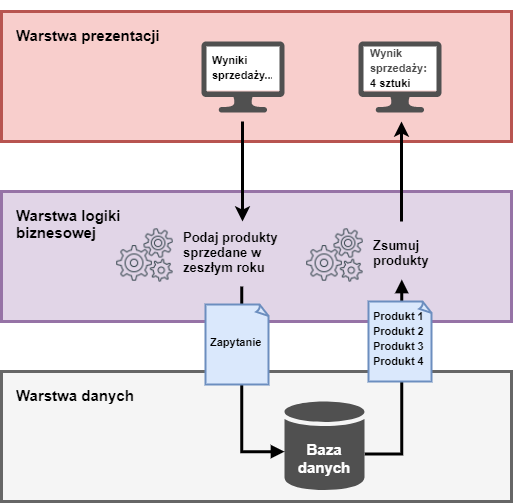
\includegraphics[width=0.7\linewidth]{graphics/three-tier-architecture.png}
	\caption{Ogólna architektura aplikacji trójwarstwowej}
	\label{three-tier-architecture}
\end{figure}

 
 Istnieją oczywiście architektury posiadające więcej warstw, jednak są one mało popularne i budowane specjalnie na potrzeby specyficznych i bardzo wymagających projektów.


\section{Warstwa prezentacji - aplikacja kliencka}

W ramach implementacji warstwy aplikacji zdecydowano się skorzystać z jednego z bardzo popularnych w ostatnich latach \textit{frameworków javascriptowych}, które dedykowane są do obsługi i komunikacji z klientem. Środowisko bibliotek javascriptowych jest obecnie bardzo szybko rozwijającym się elementem i istnieje wiele, różnego rodzaju rozwiązań tego typu. Najlepiej obecne trendy przedstawiają wykresy generowane przez system \textit{Google Trends} pokazujące popularność odpowiednich fraz w określonym przedziale czasowym. Poniżej znajduje się właśnie jeden z takich wykresów. Porównuje on zainteresowanie użytkowników sieci czterema najpopularniejszymi bibliotekami. W ramach wyjaśnienia wartości prezentowanych na osiach wykresu warto jest przytoczyć krótki tekst z instrukcji obsługi tego narzędzia:\\
\begin{quote}
    \item,,Liczby przedstawiają, jak często hasło było wyszukiwane w odniesieniu do najwyższego punktu wykresu w danym czasie i regionie. Wartość 100 oznacza najwyższą popularność hasła. Wartość 50 oznacza, że popularność hasła była dwukrotnie mniejsza. Natomiast 0 świadczy o tym, że popularność hasła wynosiła mniej niż 1\% najwyższej wartości.'' \cite{google-trends}
\end{quote}

\begin{figure}[ht]
	\centering
	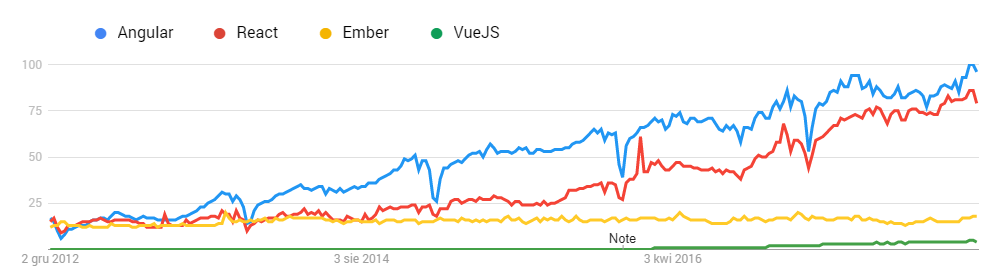
\includegraphics[width=1\linewidth]{graphics/frontend-frameworks.png}
	\caption{Porównanie popularności frameworków aplikacji klienckich}
	\label{fig:frontend-frameworks}
\end{figure}
Z przedstawionego wykresu jasno wynika, iż największym zainteresowaniem, deklasując przy tym konkurencję, cieszą się dwa rozwiązania: \textit{Angular} oraz \textit{React}, między którymi istnieje kilka zasadniczych różnic, takich jak np.: sposób wiązania danych (\textit{ang. data binding}), obsługa \textit{DOM}, czy sam fakt, że Angular jest pełnoprawnym frameworkiem, natomiast React jedynie biblioteką języka JavaScript \cite{angular-react-comparison}. Ze względu, na fakt ukierunkowania Angular'a na programowanie obiektowe (\textit{ang. Object Oriented Programming - OOP}), lepszą dokumentację oraz większą ilość materiałów naukowych, a także doświadczenie w praktycznym wykorzystaniu, zdecydowano się wybrać właśnie tę technologię.



\subsection{Framework Angular}

\quad Jest to nowoczesny i otwarty frontendowy framework oparty na języku \textbf{\textit{TypeScirpt}}, którego twórcą jest firma \textit{Google}. Głównym zadaniem biblioteki jest wdrożenie wzorca \textit{\textbf{serwis - kontroler}} w celu ułatwienia konstruowania i rozwoju aplikacji internetowych. \\
\\
Pierwsza wersja biblioteki powstała pod nazwą \textit{Angular} w roku 2009. Framework zyskał dużą popularność i przeszedł ogromną metamorfozę w stosunkowo krótkim czasie. Szybkie pojawianie się kolejnych wersji wymusiło konieczność usystematyzowania nazewnictwa. W ten sposób pierwsza wersja \textit{Angular'a} zmieniła nazwę na \textit{AngularJS}, natomiast kolejna, która pojawiła się 22 listopada 2014 roku i wprowadziła drastyczne zmiany w strukturze biblioteki przyjęła nazwę \textit{Angular 2.0}. Następna, wersja 4.0, pojawiła się 13 grudnia 2016 i przyniosła już o wiele mniej zmian i nowości w stosunku do różnic między wersją \textit{JS}, a \textit{2.0}. W momencie rozpoczynania projektu była to najnowsza wersja tej biblioteki (dokładnie \textit{4.4.6}), jednakże już 1 listopada 2017 roku pojawiła się wersja określona numerem \textit{5.0.0}, a kolejne wersje \textit{6} i \textit{7} planowane są na okres najbliższego roku. Mówiąc o ogromnej zmianie między wersjami \textit{JS}, a \textit{2.0} należy wspomnieć przede wszystkim o: różnicy w implementowanych wzorcach projektowych - \textit{AngularJS} oparty o wzorzec model-widok-controler (MVC), natomiast wersja 2.0 o model serwis-kontroler. Zmiana wzorca projektowego uniemożliwia wykonanie aktualizacji aplikacji z wersji JS na 2.0, gdyż operacja taka wymagałaby napisania całej architektury całkowicie od początku. Drugą różnicą jest wykorzystany do implementacji język \textit{Javascript} w wersji pierwszej, natomiast w wersji drugiej - \textit{Typescript}, który jest nadzbiorem \textit{Javascriptu} wspierającego budowę przejrzystszego i bardziej uporządkowanego kodu. Pomniejszych zmian i różnic między wersją \textit{JS}, \textit{2.0} i \textit{4.0} (a nawet \textit{5.0}) jest o wiele więcej i warto zapoznać się w tej kwestii z doskonałym zestawieniem autorstwa firmy \textit{Angular Minds} \cite{angular-comparison}\\
\\
Stopniowe zdobywanie popularności coraz to nowszych wersji biblioteki \textit{Angular} doskonale prezentuje kolejny wykres zapożyczony z serwisu \textit{Google Trends} przedstawiający zainteresowanie użytkowników wyszukiwarki \textit{Google} konkretnymi frazami:
\begin{figure}[ht]
	\centering
	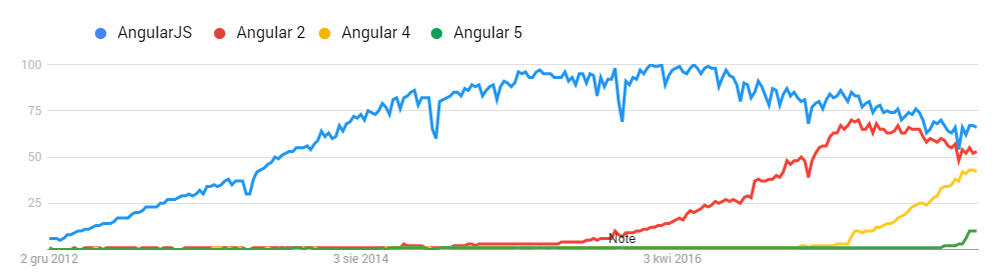
\includegraphics[width=1\linewidth]{graphics/angular-frameworks.png}
	\caption{Porównanie popularności wersji Angular'a}
	\label{fig:angular-version-comparison}
\end{figure}

W ramach wdrożenia projektu zdecydowano się na najnowszą dostępną wówczas wersję Angular'a tj. 4.4.6 umożliwiającego szybkie budowanie aplikacji typu \textit{single page}. Korzyści i możliwości jakie daje wykorzystanie tej technologii to:
\begin{itemize}
    \item Łatwość stworzenia i rozwijania projektu dzięki konsolowemu narzędziu \textbf{\textit{Angular CLI}}.
    \item Mimo stosunkowo dużego rozmiaru samej biblioteki (w porównania z konkurencyjnymi rozwiązaniami), duża wydajność działania i wiele modułów dostępnych domyślnie - bez konieczność ich dodatkowej instalacji.
    \item Dwukierunkowe wiązanie danych (\textit{ang. Two way data binding}) zapewniające automatyczną aktualizację danych modelu.
    \item Architektura i podział całego projektu na moduły ułatwiający utrzymanie kodu i tworzenie go zgodnie z regułą \textbf{\textit{DRY}} (\textit{ang. Don't repeat yourself}).
    \item Wiele wbudowanych dyrektyw skracających czas wykonywania i tworzenia podstawowych zadań.
    \item Bardzo dobra obsługa formularzy i ich walidacji ułatwiająca tworzenie aplikacji nastawionych na częste interakcje z użytkownikiem.
\end{itemize}
Ogólny zarys przepływu danych w aplikacji wygląda w ten sposób, iż głównym elementem aplikacji opartej o Angular jest \textbf{moduł}. Każda aplikacja ma przynajmniej jedną klasę modułu, który jest modułem głównym i umownie nazywany jest \textit{AppModule}. Moduły opierają się o \textbf{szablony} (\textit{ang. templates}) połączone ze znacznikami \textit{Angular'a}. Do zarządzania szablonami tworzone są klasy \textbf{komponentów}, do których wstrzykiwane są zależności (\textit{ang. \textbf{dependency injection}}) zawierające logikę aplikacji w postaci \textbf{serwisów} (\textit{ang. services}). Angular generuje i przetwarza strukturę dokumentu DOM zgodnie z instrukcjami reprezentowanymi przez \textbf{dyrektywy}.  Ostatnim kluczowym elementem są \textbf{metadane}, które informują Angular'a, iż dany element jest np. komponentem lub dyrektywą. Graficzne przedstawienie architektury Angular'a przedstawia \textit{rysunek 3.4}.

\begin{figure}[ht]
	\centering
	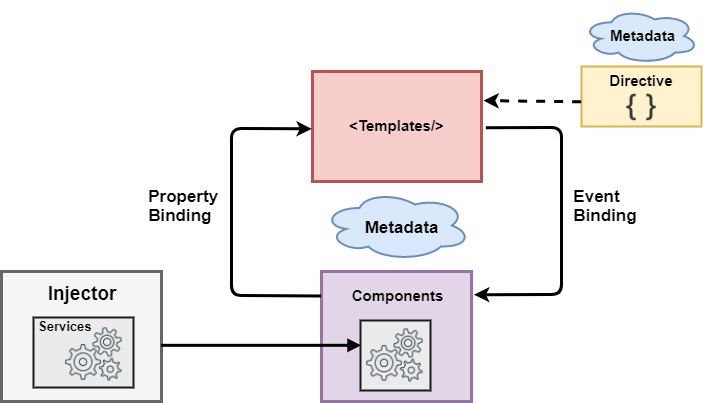
\includegraphics[width=1\linewidth]{graphics/angular-architecture.png}
	\caption{Ogólna architektura frameworka Angular 4}
	\label{fig:general-angular-architecture}
\end{figure}

	\subsubsection{Angular CLI}
\quad Wspomniane już wcześniej, jako jedna z licznych zalet Angular'a, narzędzie \textbf{Angular CLI} to konsolowy interfejs służący do budowania, utrzymania, rozwijania i konfigurowania aplikacji stworzonych właśnie w tej technologii. W ostatnim czasie stało się jednym z najczęściej wykorzystywanych narzędzi do tego typu zadań. 
Usprawnia ono proces budowania nowego projektu ograniczając konieczność wykonania wielu niełatwych i powtarzalnych czynności do jednej konsolowej komendy. Przykładem może być polecenie tworzące nowy projekt: 
\begin{lstlisting}
    ng new [name]
\end{lstlisting}
Po wykonaniu tej komendy zostaje wygenerowany podstawowy szablon, który jest gotowy do uruchomienia za pomocą komendy:
\begin{lstlisting}
    ng serve
\end{lstlisting}
Dzięki tym dwóm prostym komendom został stworzony i uruchomiony w pełni funkcjonalny projekt aplikacji, oszczędzając w ten sposób programiście kilku godzin żmudnych ustawień i konfiguracji.\\
Angular CLI nie ogranicza się jednak jedynie do generowania projektu. Jest również bardzo przydatne w czasie jego rozwoju, np. przy pomocy jednej komendy generując wszystkie potrzebne pliki dla nowego komponentu czy modułu:
\begin{lstlisting}
    ng generate component [name]
    ng generate module [name]
\end{lstlisting}

	\subsubsection{Komponent ng2-file-upload}
	\quad Omawiając wszystkie ważne składowe aplikacji klienckiej, koniecznie należy wspomnieć o jednym z komponentów, który ma zostać wykorzystany w aplikacji \textit{PhotoLab}.\\
	\textbf{Ng2-file-upload} jest doskonałym przykładem jednego z bardzo wielu gotowych i ogólnodostępnych komponentów (na odpowiedniej licencji: np. MiT) dedykowanych dla frameworka Angular. Ogromna ilość komponentów wskazuje na wspominane wcześniej bardzo szeroko rozwinięte \textit{community}. Posiadanie grona takich osób dla każdej technologii jest bardzo ważne, gdyż gwarantuje: 
	\begin{itemize}
	    \item Szerokie wsparcie w przypadku problemów - programiści oferują wzajemną pomoc w rozwiązywaniu problemów i dzielą się własnym doświadczeniem.
	    \item Ogromną ilość materiałów, poradników i szkoleń dostępnych w Internecie, które pozwalają w przyjazny sposób zaznajomić się z konkretnymi zagadnieniami.
	    \item Szybki rozwój (w przypadku Angular'a jest bardzo dobrze widoczne) i aktualność z panującymi trendami, a wręcz bycie ich prekursorem.
	\end{itemize}
	\textit{ng2-file-upload} to stworzony przez jednego z członków społeczności i udostępniony na licencji \textit{MIT} komponent odpowiedzialny za obsługę wgrywania plików. Oferuje on bardzo przystępny interfejs użytkownika z uwzględnieniem takich elementów jak:
	\begin{itemize}
	    \item Wybór plików za pomocą standardowego okna systemowego lub zasady przeciągnij i upuść (\textit{ang. drag and drop}).
	    \item Wypisanie wybranych plików gotowych do wgrywania.
	    \item Możliwość wgrywania wszystkich wybranych plików jednocześnie.
	    \item Animowany pasek postępu procesu przesyłania.
	\end{itemize}
	Aby system ten sprostał wymaganiom \textit{PhotoLab} wystarczy wprowadzić do niego kilka modyfikacji takich jak np.: dołączenie podglądu wybranych zdjęć, czy ograniczenie opcji przesyłania plików jedynie do wszystkich jednocześnie. Należy również zaznaczyć, iż komponent ten działa jedynie w warstwie prezentacji, co oznacza, iż konieczne jest zaimplementowanie obsługi uzyskanych informacji (czyli zapisanie plików i informacji o nich) po stronie serwera aplikacji.
	% Komponent umożliwiający obsługę dynamicznego wgrywania zdjęć

\subsection{Bootstrap}
\quad Warstwa aplikacji to nie tylko interfejs przysyłający dane do kolejnej warstwy. To również, a wręcz przede wszystkim interakcja z użytkownikiem systemu, który chce skorzystać z usług firmy. Bardzo ważnym aspektem jest więc zaprezentowanie danych i funkcjonalności w sposób estetyczny, usystematyzowany i przyjazny dla człowieka. Do tego celu służą właśnie kaskadowe arkusze stylów (\textit{ang. cascading style sheets (CSS)}), które opisują formę prezentacji struktury utworzonej w hipertekstowym języku znaczników (\textit{ang. HyperText Markup Language}), czyli popularnym HTML'u. Czasy, gdy całe strony i duże aplikacje internetowe były dekorowane jedynie przy pomocy czystego CSS dawno minęły. Obecnie na szeroką skalę wykorzystuje się \textbf{\textit{frameworki CSS}}, czyli biblioteki zawierające zestaw wielu gotowych narzędzi i komponentów ułatwiających tworzenie estetycznych i przejrzystych interfejsów stron internetowych. \\
\\
Jednym z takich rozwiązań jest \textbf{\textit{Bootstrap}}. Jest to obecnie, podobnie jak Angular, najpopularniejsze i najszerzej wykorzystywane narzędzie w swojej klasie charakteryzujące się bardzo prężnym rozwojem. Zespołem odpowiedzialnym za Bootstrapa są programiści \textit{Twitter'a}. 10 sierpnia 2017 roku opublikowali oni najnowszą wersję 4.0.0 beta 2, która to właśnie wersja zostanie wdrożona w aplikacji \textit{PhotoLab}. Argumentami za zastosowaniem technologii znajdującej się jeszcze w wersji beta była przede wszystkim jej bardzo dobra stabilność (jak na wersję beta), szerokie grono społeczności, dobra dokumentacja, a przede wszystkim różnice względem poprzedniej wersji (3.3.7):
\begin{itemize}
    \item pliki źródłowe tworzone w technologi \textit{SASS}, a nie \textit{LESS},
    \item domyślna jednostka, \textit{rem} - czyli wysokość czcionki elementu korzenia w drzewie dokumentu, a nie piksel,
    \item pięcio-, a nie czterowarstwowy \textit{grid}, czyli siatka, według której budowany jest szablon,
    \item wbudowany nowy sposobu układania elementów na stronie - \textit{FlexBox}.
\end{itemize}
Powodem wyboru \textit{Bootstrapa} jako frameworka CSS jest jego dobra znajomość i doświadczenie w wykorzystaniu, co znacznie ułatwi i przyspieszy pracę nad aplikacją ale przede wszystkim bardzo estetyczny sposób prezentowania treści w formie, która w pełni zadowala właściciela laboratorium.

\section{Warstwa logiki biznesowej - serwer aplikacji}

\quad Bardzo ważną częścią przygotowywania projektu jest podjęcie decyzji o wyborze technologii dla warstwy aplikacji, czyli warstwy najważniejszej dla całego modelu trójwarstwowego. W tej płaszczyźnie bowiem wykonywane są najistotniejsze operacje obsługujące procesy biznesowe, takie jak wyliczenia, autoryzacja użytkowników czy dostęp do danych. Podejmując decyzje należy mieć na względzie postawione cele tj. bezpieczeństwo aplikacji, jej wydajność i dostępność oraz możliwie niskie koszty wdrożenia i utrzymania. \\
\\
Możliwości i technologii jest wiele. Jedne są bardziej odpowiednie, inne mniej. Ścisła czołówka tzw. \textit{aplikacji backendowych} to z pewnością technologie takie jak: \textit{PHP}, \textit{.NET} i \textit{Java}, jednak coraz większą popularność zyskują również: \textit{Python} czy \textit{Ruby}.\\
Wybór nie jest łatwy. Żadne zweryfikowane przesłanki zewnętrzne takie jak szybkość, wydajność, czy bezpieczeństwo nie wskazują konkretnego faworyta tej konkurencji. Wybór technologi, w której zostanie zaimplementowana aplikacja został więc wybranych w oparciu o aspekt wewnętrzny jakim są predyspozycje autora. W ramach implementacji warstwy biznesowej aplikacji \textit{PhotoLab} wykorzystana zostanie technologia \textbf{ASP.NET Core}.

\subsection{ASP.NET Core}
\textbf{\textit{.NET Framework}} jest to platforma programistyczna wywodząca się z rodziny rozwiązań firmy \textit{Mircosoft}.  Dostarcza wiele standardowych funkcjonalności w postaci \textbf{bibliotek klas} oraz przede wszystkim \textbf{środowisko uruchomieniowe} (\textit{ang. Common Language Runtime} (\textit{CLR}). \\
Technologia ta nie jest związana z żadnym konkretnym językiem programowania i umożliwia budowanie kodu w oparciu o jeden z bardzo wielu dostępnych, m.in. C++, C\# czy F\#. Platforma \textit{\textbf{ASP.NET}} to, podobnie jak \textit{ADO.NET} (używana jako narzędzie dostępu do danych), pochodna platformy \textit{.NET} służąca do budowania dynamicznych strony WWW. \\
    \textbf{\textit{ASP.NET Core}} jest biblioteką aplikacji internetowych, który wchodząc na rynek w połowie 2016 roku w wersji \textit{1.0} wprowadził ogromną rewolucję w produktach z serii \textit{ASP.NET}: 
    \begin{enumerate}
        \item Zintegrował wszystkie trzy osobno występujące modele aplikacji internetowych, czyli:
    \begin{itemize}
        \item \textit{ASP.NET MVC} - bibliotekę implementującą wzorzec \textit{Model-View-Controller} (\textit{MVC}) w aplikacjach internetowych.
        \item \textit{ASP.NET Web API} - strukturę typu \textit{HTTP API} służącą do budowania \textit{web serwisów}.
        \item \textit{ASP.NET Web Pages} - platformę wykorzystującą jedynie strony oparte o  składnię \textit{Razor}.
    \end{itemize}
   \item Został całkowicie przebudowany i stworzony w zupełnie nowym stosie technologicznym, zachowując przy tym jednak bardzo duże podobieństwo konceptualne z \textit{ASP.NET MVC}.
    \item Jego całkowite przebudowanie umożliwiło:
        \begin{itemize}
            \item stworzenie wieloplatformowej technologii dostępnej już nie tylko na systemy \textit{Windows}, ale również \textit{Linux} i \textit{Mac},
            \item zbudowanie modularnej biblioteki opartej o paczki \textit{NuGet'owe},
            \item udostępnienie oprogramowania na otwartej licencji \textit{MiT}, która nakierowana jest na rozwój społecznościowy,
            \item zunifikowanie sposobu generowania interfejsów internetowych,
            \item całkowite przyspieszenie działania całej platformy względem jej poprzednich wersji,
            \item stworzenie nowego, bardzo lekkiego i modułowego potoku żądań HTTP (\textit{ang. request pipeline}).
        \end{itemize}
    \end{enumerate}
    Kierując się wszystkimi wspomnianymi powyżej przesłankami, została podjęta decyzja o wdrożeniu projektu aplikacji internetowej (ASP.NET Core Web Application) o strukturze typu \textbf{\textit{Web API}} w najnowszej obecnie wersji \textbf{\textit{1.1}}.\\
    \\
    Poniżej (\textit{rys. 3.5}) przedstawiony został ogólny zarys
    obsługi żądań zapytań HTTP docierających do warstwy biznesowej aplikacji opartej o technologię ASP.NET Core Web API i obsługującej połączenie z bazą danych poprzez narzędzie \textit{Entity Framework}.

    \begin{figure}[ht]
	\centering
	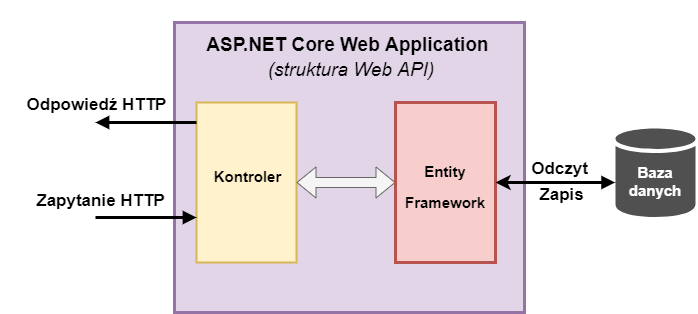
\includegraphics[width=1\linewidth]{graphics/asp-net-web-api-architecture.png}
	\caption{Architektura i przepływ danych warstwy biznesowej}
	\label{fig:asp-net-web-api-architecture}
    \end{figure}

\subsection{ASP Identity i JSON Web Token}
    W celu zapewnienia zakładanego, wysokiego poziomu bezpieczeństwa zarówno klientów systemu jak i przechowywanych w nim danych, konieczne jest zaimplementowanie systemu weryfikującego użytkowników. Zanim jednak zostanie omówione wybrane rozwiązanie należy wyjaśnić kilka pojęć związanych z tą tematyką.\\
    \\
    Z kwestią bezpieczeństwa nierozerwalnie związane są trzy pojęcia, które często są mylone i niepoprawnie definiowane. Istnieje wiele definicji i wywodów na temat każdego z poniższych haseł, jednak najprostsze wyjaśnienia przedstawiają się następująco:
    \begin{itemize}
        \item \textbf{Identyfikacja} (\textit{ang. identity}) - rozpoznanie użytkownika, próbującego połączyć się z systemem.
        \item \textbf{Uwierzytelnienie} (\textit{ang. authentication}) - upewnienie co najmniej jedenej ze stron o tożsamości drugiej. Jest to tak naprawdę identyfikacja na poziomie zaawansowania i szczegółowości pozwalającej na przyznanie odpowiednich uprawnień i dostępów.
        \item \textbf{Autoryzacja} (\textit{ang. authorization}) - jest to zapewnienie stronie zgłaszającej taką potrzebę odpowiednich uprawnień i praw dostępu. 
    \end{itemize}
    Podsumowując: ,,identyfikacja, uwierzytelnianie i autoryzacja powinny być elementami każdej transakcji biznesowej i muszą być zagwarantowane przez system komunikacyjny i oprogramowanie pośredniczące w związkach pomiędzy dostawcami i klientami.'' \cite{identity-theory}\\
    \\
    Cały system weryfikacji użytkowników można zaimplementować samodzielnie od podstaw. Mija się to jednakże z celem w momencie, gdy platforma \textit{.NET} udostępnia świetne narzędzie jakim jest \textbf{\textit{ASP.NET Identity}}. Dlaczego warto wybrać akurat to, gotowe rozwiązanie? Z pewnością dlatego, iż cały system weryfikacji użytkowników jest procesem trudnym i skomplikowanym, a najmniejsza luka w jego implementacji powoduje pojawienie się tzw. najsłabszego ogniwa, które powoduje, iż inne, nawet najmocniejsze zabezpieczenia tracą swoją wartość. \textit{ASP.NET Identity} jest produktem rozwijanym i modyfikowanym od wielu lat, uwzględniane są w nim wszystkie najnowsze mechanizmy, zabezpieczenia, sugestie użytkowników oraz dostrzeżone błędy i uchybienia. Gotowy system, stworzony przez duży zespół wsparty ogromnym \textit{community}, wykorzystany i przetestowany na setkach tysięcy rozwiązań i systemów, zarówno mniejszych, jak i większych, jest idealnym wyborem dla zapewnienia bezpieczeństwa aplikacji \textit{PhotoLab}.\\
    \\
    Mimo wielu zalety, dostrzeżono również dwa poważne mankamenty tego rozwiązania. Biblioteka ta działania jedynie w drugiej warstwie modelu - warstwie biznesowej. Oznacza to, iż sesje zalogowanego użytkownika muszą być przetrzymywane na serwerze, co powoduje jego dodatkowe obciążenie. Drugi przypadek zakłada dalszy rozwój aplikacji i pojawienie się dodatkowych serwisów, np. do obsługi urządzeń mobilnych. W takim przypadku konieczna jest ponowna implementacja systemu weryfikacji użytkownika na kolejnym serwerze i przez to redundancja kodu i odpowiedzialność. Rozwiązaniem tego typu problemów jest uzupełnienie biblioteki \textit{ASP.NET Identity} o standard kluczy dostępu \textbf{\textit{JSON Web Token}}.\\
    Jest to otwarta technika generowania kluczy uwzględniających prawa dostępu. Zasada jej działania oparta jest na zasadzie klucza prywatnego. Niepowtarzalny klucz JWT generowany jest w momencie logowania użytkownika i składa się z trzech części:
    \begin{itemize}
        \item nagłówka (\textit{ang. header}) - zawierającego informacje o typie klucza JWT oraz sposobie jego szyfrowania,
        \item ładunku (\textit{ang. payload}) - jak sama nazwa wskazuje, przechowującego informacje na temat praw dostępów, czy np. czasu ważności tokenu,
        \item podpisu (\textit{ang. signature}) - do którego utworzenia konieczne są dwie pozostałe części, które zabezpieczone są poprzez sekretny klucz aplikacji i szyfr ustalony w nagłówku.
    \end{itemize}
    Klucz generowany jest po stronie serwera aplikacji i zwracany do warstwy klienckiej, w której może być przetrzymywany, np. w pamięci lokalnej. W momencie odwołania się użytkownika do zabezpieczonej warstwy biznesowej, wraz z zapytaniem przesyła on klucz JWT, który jest jedynie weryfikowany i w razie sukcesu otwiera dostęp do zasobów / funkcjonalności lub w razie niepowodzenia serwer zwraca odpowiedź z kodem błędu 403.\\
\\
Zastosowanie kluczy JWT rozwiązuje dwa wcześniej wymienione problemy pojawiające się w momencie korzystania z modułu \textit{Identity}. Po pierwsze ciężar zapamiętania sesji logowania przerzuca na aplikację kliencką, odciążając w te sposób serwer, który nie musi już przetrzymywać w swojej pamięci bazy zalogowanych użytkowników. Po drugie mechanizm autoryzacji może zostać zaimplementowany na jednym z obsługujących aplikację serwerów, do którego użytkownik zawsze będzie się odnosił wyłącznie w momencie logowania. Pozostałe moduły będą musiały jedynie sprawdzić poprawność otrzymanego klucza i udostępnić swoje zasoby. Opisaną sytuację doskonale przedstawia diagram (\textit{rys. 3.6}):
    
    
    \begin{figure}[ht]
	\centering
	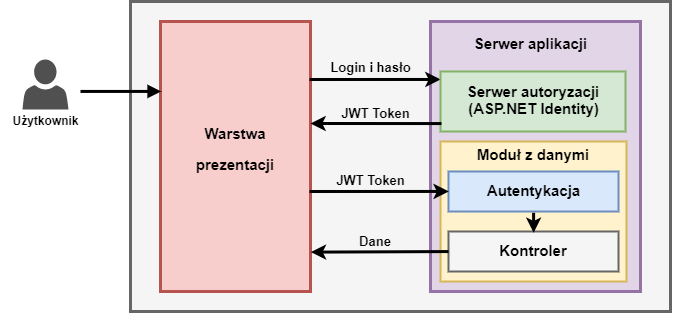
\includegraphics[width=1\linewidth]{graphics/jwt-identity-diagram.png}
	\caption{Weryfikacja użytkownika z użyciem ASP.NET Identity i JSON Web Token}
	\label{fig:jwt-identity-diagram}
    \end{figure}




\section{Warstwa danych - baza danych}
    Ostatnim elementem modelu trójwarstwowego aplikacji jest warstwa danych.
    Najczęściej można ją opisać jako swoisty pojemnik na informacje. Powinien on zapewniać bezpieczeństwo i trwałość swojej zawartości oraz łatwą i szybką jej dostępność. \\
    \\
    Istnieje obecnie wiele rodzajów baz danych, które różnią się względem siebie sposobem przetrzymywania informacji. Wybrane z nich to bazy:
    \begin{itemize}
        \item Proste (kartotekowe) - tablica danych skonstruowana jest jako samodzielny dokument, który nie może wchodzić w związki z innymi tablicami. Przykładami implementacji takiej bazy mogą być: książki telefoniczne, książki kucharskie czy różnego rodzaju spisy.
        \item Relacyjne (RDB) - dane przetrzymywane w postaci encji umieszczonych w tabelach, które z kolei mogą wchodzi w relacje między sobą. Posiadają predefiniowane typy oraz wewnętrzne języki programowania (\textit{SQL}). Przykładami są bazy: \textit{Oracle}, \textit{Ingress}, \textit{Access}, \textit{MySQl} czy \textit{MS SQL}. Obecnie dominujący typ danych w zastosowaniach komercyjnych (ok. 95\% rynku).
        \item Obiektowe (ODB) - nie zdefiniowane żadnym oficjalnym standardem. Ich podstawowym zadaniem jest odwzorowanie obiektów i powiązań wchodzących w skład aplikacji na identyczne w bazie danych. Łączą one właściwości obiektowości i obiektowych języków programowania wraz z możliwościami systemów bazodanowych.
        \item Nierelacyjne (NoSQL) - nie posiadają ściśle zdefiniowanej struktury. Dane składowane jako dokumenty - np. w formie \textit{JSON}. Charakteryzują się dużą skalowalnością i wydajnością. Przykładamy implementacji tego typu baz są: \textit{MongoDB} oraz \textit{Apache Cassandra}.
    \end{itemize}
    Najbardziej naturalnym i najczęstszym wyborem w przypadku konstruowania warstwy pośredniej w technologii \textit{ASP.NET} jest zbudowanie środowiska bazodanowego w oparciu o produkt pochodzący z tej samej rodziny - firmy Microsoft - jakim jest \textbf{\textit{Microsoft SQL Server}}. Połączenie, dodatkowo wzbogacone o narzędzie klasy \textbf{\textit{ORM}} - \textit{\textbf{Entity Framework}} - stawowi doskonały pakiet zapewniający najlepsze możliwe połączenie warstwy aplikacji i warstwy danych modelu trójwarstwowego.
    
    Wykorzystanie relacyjnej bazy danych daje wszystkie możliwe korzyści wynikające z przechowywania danych w takiej strukturze tj.: możliwość stosowania złożonych kryteriów wyszukiwania, bardzo dobre mechanizmy dostępu do danych, a także pewną i sprawdzoną strukturę przetestowaną w wielu możliwych scenariuszach i przypadkach. Nie jest być może to struktura najszybsza, ani najbardziej podatna na skalowalność, jednakże w aplikacji \textit{PhotoLab} nie są to kryteria najważniejsze. Bardzo dużą zaletą i ułatwieniem w operowaniu na bazie relacyjnej typu \textit{MS SQL}, gdzie reprezentacja danych nie zawsze jest przyjazna i naturalna, jest narzędzie służące do mapowania obiektowo-relacyjnego. Zdecydowania ułatwia to pracę nad aplikacją oraz przyspiesza jej rozwój. Wykorzystując narzędzia typu \textit{ORM}, czasami mogą pojawiać się problemy wydajnościowe, jednak w przypadku projektowanej aplikacji nie przewiduje się takowych, tak więc liczba zalet zdecydowanie przewyższa wady wprowadzenia tego rozwiązania.
    
\subsection{Microsoft SQL Server}
    System służący do zarządzania bazą danych, którego twórcą jest firma \textit{Microsoft}. Jest to flagowy produkt tej korporacji w zakresie operacyjnych systemów zarządzania bazami danych (\textit{ang. Operational Database Management Systems (ODBMS)}.\\
    \\
    Podstawą platformy \textit{SQL Server} jest usługa serwera (\textit{ang. database engine}), który realizuje wszystkie zadania dotyczące obsługi i utrzymania bazy danych. Całe środowisko \textit{SQL Server} jest skalowalne, w zależności od potrzeb i wymagań może składać się z wielu różnych komponentów. Na jednym serwerze (fizycznym, bądź wirtualnym)  możliwa jest instalacja wielu \textit{instancji} środowiska \textit{SQL Server}. Ta z kolei może zarządzać wieloma \textit{bazami danych}. Zazwyczaj jednak poprzez względy wydajnościowe na jednym serwerze instaluje się jedną instancję z maksymalnie dwoma lub trzema bazami danych.\\
    \\
    Kilka najbardziej podstawowych i oferowanych przez \textit{SQL Serwer} komponentów to:
    \begin{itemize}
        \item Wspomniany wcześniej \textit{silnik bazy danych}.
        \item \textit{Usługi raportujące} jako gotowy system oparty o technologię .NET do generowania raportów z bazy danych.
        \item \textit{Usługi analityczne} w skład których wchodzi kilka narzędzie analitycznych głównie z zakresu \textit{Business Intelligence}, czyli przetwarzania danych w informacje, by następnie wyciągnąć z nich odpowiednie wnioski i wiedzę.
        \item \textit{Usługi integracji danych} oferujące możliwość zbierania i analizy danych z różnych źródeł. 
    \end{itemize}
    Omawiając pakiet bazodanowy Microsoft należy również wspomnieć o udostępnionych w ramach niego narzędziach takich jak: \textbf{SQL Server Profiler} i \textit{\textbf{SQL Server Management Studio}}. Drugie przedstawione narzędzie zostanie wykorzystane w ramach wdrożenia projektu w celu: administracji, przeglądu i edycji danych w \textit{graficznym środowisku użytkownika} (\textit{GUI}).
    
    \subsection{Entity Framework Core}
    Entity Framework podobnie jak \textit{SQL Server Management Studio} należy do technologii z rodziny \textit{.NET}, a konkretnie \textit{ADO.NET}, a więc jest doskonale zintegrowane do obsługi bazy danych \textit{Microsoft SQL} oraz aplikacji \textit{ASP.NET}.
    \\
    \\
    Jest to narzędzie typu ORM (ang. Object-relational mapping), czyli takie, które odwzorowuje obiekty architektury obiektowej na tabele i encje w relacyjnej bazie danych. Odwzorowanie takie ma bardzo dobre zastosowanie w przypadku tworzenia systemu zorientowanego na podejście obiektowe, natomiast baza danych operuje na relacjach. Programiści w momencie zajmowania się danymi, mogą pracować na wyższym poziomie abstrakcji, przez co generują mniejszą ilość redundantnego kodu i ciągle pozostają w sferze programowania obiektowego, a nie zorientowanego na tabele i encje.
\chapter{Projekt systemu}
	\section{Struktura}
	\section{Serwer aplikacji i API}
		\subsection{Wzorzec projektowy}
		\subsection{Przetwarzanie zapytań}
		\subsection{Baza danych}
	\section{Aplikacja internetowa}
		\subsection{Single Page Application}
		\subsection{Framework}
		\subsection{Moduły}
			\subsubsection{Moduł Administratora}
			\subsubsection{Moduł Laboratorium}
		\subsection{Warstwa prezentacji}
	\section{Środowisko produkcyjne}
		\subsection{Proces instalacji}
		\subsection{Uruchomienie}
		\subsection{Użytkowanie}
		
		Luźno wrzucone diagramy aplikacji:
\begin{figure}[ht]
	\centering
	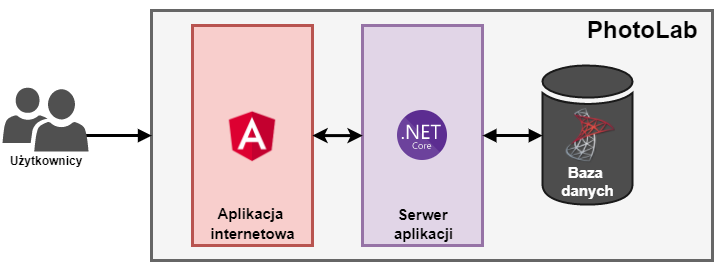
\includegraphics[width=0.7\linewidth]{graphics/general-application-architecture.png}
	\caption{Ogólny diagram architektury aplikacji \textit{PhotoLab}}
	\label{fig:general-application-architecture}
\end{figure}

\begin{figure}[ht]
	\centering
	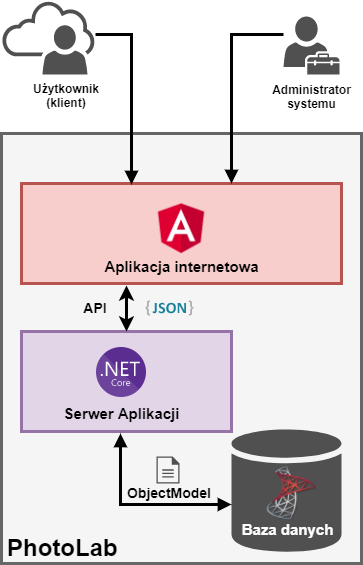
\includegraphics[width=0.5\linewidth]{graphics/application-architecture-without-payu.png}
	\caption{Szczegółowy diagram architektury aplikacji \textit{PhotoLab}}
	\label{fig:application-architecture-without-payu}
\end{figure}

\begin{figure}[ht]
	\centering
	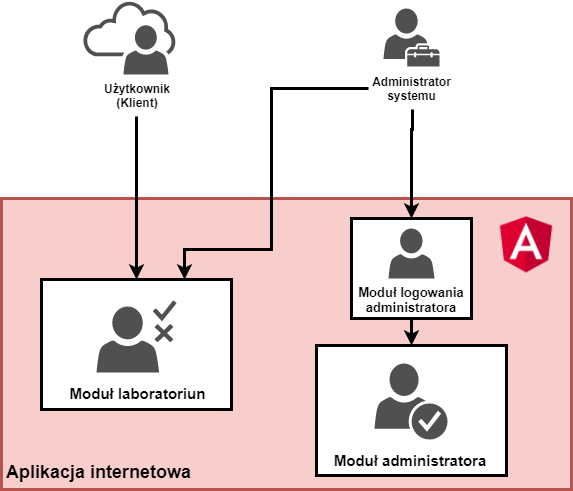
\includegraphics[width=0.5\linewidth]{graphics/client-architecture.png}
	\caption{Szczegółowy diagram architektury aplikacji klienckiej}
	\label{fig:client-architecture}
\end{figure}
\chapter{Testowanie}

\section{Zgodność z wymaganiami}
\section{Testy funkcjonalne}
\section{Testy użyteczności}
\section{Testy wydajnościowe}


\chapter{Podsumowanie}
\section{Efekt końcowy}
\section{Możliwości dalszego rozwoju aplikacji}
\section{Wnioski}


\appendix
\chapter{Opis załączonej płyty CD}
Tutaj jest miejsce na zamieszczenie opisu zawartości załączonej płyty.
Należy wymienić, co zawiera.


%\bibliographystyle{plalpha}
\bibliographystyle{plabbrv}

%UWAGA: bibliotekę referencji należy przygotować samemu. Dobrym do tego narzędziem jest JabRef.
%       Nazwę przygotowanej biblioteki wpisuje się poniżej bez rozszerzenia 
%       (w tym przypadku jest to "dokumentacja.bib")
\addcontentsline{toc}{chapter}{Bibliography}
\bibliography{dokumentacja}

\chapterstyle{noNumbered}
\phantomsection % sets an anchor
\addcontentsline{toc}{chapter}{Indeks rzeczowy}
\printindex


\newpage
\mbox{}\pdfbookmark[0]{Spis rysunków}{spisRysunkow.1}
%\addcontentsline{toc}{chapter}{Spis rysunków}
\listoffigures*
\begin{flushleft}

\end{flushleft}
%{%
%\let\oldnumberline\numberline%
%\renewcommand{\numberline}{\figurename~\oldnumberline}%
%\listoffigures%
%}


\newpage
\mbox{}\pdfbookmark[0]{Spis tabel}{spisTabel.1}
%\addcontentsline{toc}{chapter}{Spis tabel}
\listoftables*

\chapter*{Słownik pojęć i skrótów}\mbox{}\pdfbookmark[0]{Słownik pojęć i skrótów}{skroty.1}
\label{sec:skroty}
\noindent
\begin{description}
  \item [SPA] (ang.\ \emph{Single Page Application})
  \item [MVC] (ang.\ \emph{Model-View-Controller})
  \item [DOM] (ang.\ \emph{Document Object Model})
  \item [OOP] (ang.\ \emph{Object Oriented Programming})
  \item [DRY] (ang.\ \emph{Don't Repeat Yourself})
  \item [CLR] (ang.\ \emph{Common Language Runtime})
  \item [ORM] (ang.\ \emph{Object-Relational Mapping})
  
  
%  \item [Licencja MIT]
%  \item [PhotoLab]
%  \item [Framework] 
%  \item [Frontend]
% \item [Backend]
%  \item [Community]
\end{description}
 %skróty można sobie pominąć


\end{document}
